\documentclass[a4paper,10pt]{article}
\usepackage{tikz}
\usetikzlibrary{%
  calc,%
  decorations.pathreplacing,%
  fadings,%
  shadings%
}
\renewcommand*{\familydefault}{\sfdefault}

\begin{document}

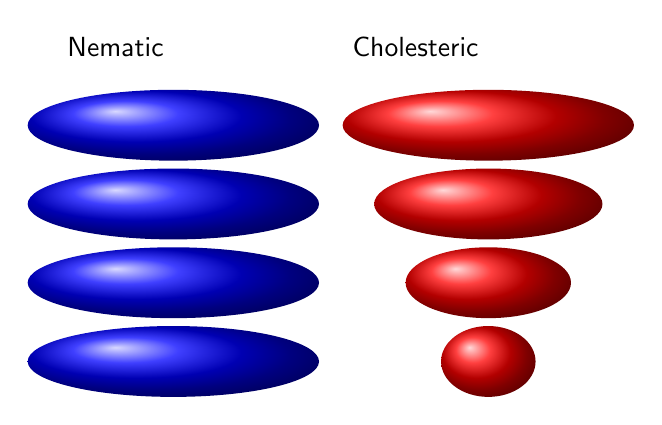
\begin{tikzpicture}
  \def\nuPi{3.1459265}

  \shade[ball color=red] (12, 9) ellipse(0.60 and 0.45);
  \shade[ball color=red] (12,10) ellipse(1.05 and 0.45);
  \shade[ball color=red] (12,11) ellipse(1.45 and 0.45);
  \shade[ball color=red] (12,12) ellipse(1.85 and 0.45);

  \draw(12, 13) node[left] {Cholesteric};

  \shade[ball color=blue] (8, 9) ellipse(1.85 and 0.45);
  \shade[ball color=blue] (8,10) ellipse(1.85 and 0.45);
  \shade[ball color=blue] (8,11) ellipse(1.85 and 0.45);
  \shade[ball color=blue] (8,12) ellipse(1.85 and 0.45);

  \draw(8, 13) node[left] {Nematic};


\end{tikzpicture}
\end{document}
